\documentclass[9pt,twocolumn,twoside]{styles/osajnl}
\usepackage{fancyvrb}
\journal{nist} 

\usepackage{titlesec}

\usepackage{ifxetex}
\ifxetex
\usepackage{fontspec}
\setmainfont[Mapping=tex-text]{STIXGeneral}
\else
\usepackage[T1]{fontenc}
\usepackage[utf8]{inputenc}
\fi
\usepackage{textcomp}
\usepackage{fancyvrb}
\usepackage{graphicx}
\usepackage{array}
\usepackage{ulem}
\usepackage{amssymb}
%\usepackage{fancyhdr}
%\renewcommand{\headrulewidth}{0pt}
%\renewcommand{\footrulewidth}{0pt}
\usepackage{color}
\usepackage{xcolor,colortbl}
\newcommand{\grey}{\cellcolor{lightgray}}  %{0.9}
\newcommand{\blue}{\cellcolor{gray}}  %{0.9}

\usepackage{hyperref}
\usepackage{url}

\usepackage{enumitem}
\setlist{nosep}

\usepackage{csvsimple}
%\usepackage{longtable}
%usepackage{lscape}
%\usepackage{booktabs}
\usepackage{pifont}
\usepackage{fancyvrb}
\usepackage{listings}
\usepackage{lstautogobble}

\lstset{basicstyle=\ttfamily,
%\lstset{basicstyle=helvetica,
  mathescape=true,
  escapeinside=||,
  autogobble}

\newcommand*\rot{\rotatebox{90}}
\newcommand*\OK{\ding{51}}
\newcolumntype{L}{>{\centering\arraybackslash}m{4cm}}
\usepackage{xcolor}
\usepackage[colorinlistoftodos,prependcaption,textsize=normalsize]{todonotes}
\usepackage[justification=centering]{caption}




\setcounter{secnumdepth}{4}

\titleformat{\paragraph}
{\normalfont\normalsize\bfseries}{\theparagraph}{1em}{}
\titlespacing*{\paragraph}
{0pt}{3.25ex plus 1ex minus .2ex}{1.5ex plus .2ex}



\title{NIST Report 2017-01-20}

\author[1]{Badi' Abdul-Wahid}
\author[1]{Hyungro Lee}
\author[1]{Gregor von Laszewski}
\author[1,*]{Geoffrey Fox}

\affil[1]{School of Informatics and Computing, Bloomington, IN 47408, U.S.A.}

\affil[*]{Corresponding authors: gcf@indiana.edu}

\dates{\today}

\ociscodes{Cloud, Big Data}

\doi{\url{https://github.com/cyberaide/nist-report}}


\begin{abstract}
FIXME
\end{abstract}

\setboolean{displaycopyright}{true}

\begin{document}

\maketitle

%%%%%%%%%%%%%%%%%%%%%%%%%%%%%%%%%%%%%%%%%%%%%%%%%%%%%%%


\section{Overview}

This document summarizes the NIST Big Data Public Working Group
(BDPWG) use-cases document: "Possible Big Data Use Cases
Implementation using NBDRA". Additional projects originated from
classes taught at Indiana University.


The focus of our current work is the development of abstractions
capturing the basic concepts we have seen and the development of a
REST API implementing some of these ideas. We describe a few of the
underlying components for allocating and managing virtual
clusters. Additionally, a summary of the ecosystem (Open Source via
GitHub) and Academic (via Indiana University classes) in which Big
Data Software is used. There is a brief description of a few of the
Use Cases, as well as a description of the major components. Finally
we describe the software stacks developed as part of this work and
then conclude with some lessons learned and ideas for future work.



\section{Summary of Changes from Last Update}

Previous update described FIXME.  Since then, we have begun
development of an API with a REST frontend for bringing up and
deploying several of the technologies used by the Use Cases



\subsection{Plugins}

Previously we were developing a single Ansible repository with the
software modules such as Spark, HBase, Drill, etc. We have come to
understand that an improved approach is to support a plugin-based
architecture for deployment components. These components can therefore
more easily be integrated from various sources.


\subsection{Deployers}

We had previouly settled on the use of Ansible for deploying software
components. While Ansible continues to be the primary tool, we are
designing in support for other systems as well. This would allow users
more familiar with Chef or NixOps for example to take advantage of the
domain they know better.



\subsection{Stack Compositions}

Compositions will allow different deployers to build on top of each
other.




\section{Focus of Current Work}

We are currently working on developing a an API for managing the
infrastructure and deploying software stacks to the cluster. This API
will be exposed as a REST service. A preliminary set of components
that has been developed as part of the API has been used by students
in classes in the Fall of 2016 and expect even more to use these
components in the Spring 2017 class~\cite{www-i524}.


\section{Architecture}

To address the complexity of the development of the different roles
and scripts users must not only deliver them and present them to the
data scientists, but must be prepared based on DevOps founded
principals that deploys and test the scripts in a continuous or on an
on demand fashion (in case significant resources are used to test the
application). Hence in addition to the development of the scripts to
deploy the software, we must also develop scripts that automatically
execute the application on existing data sets to verify the
functionality upon changes in the application, data, operating system,
or infrastructure services such as hypervisors and containers.


\begin{figure}[htb]
  \centering
      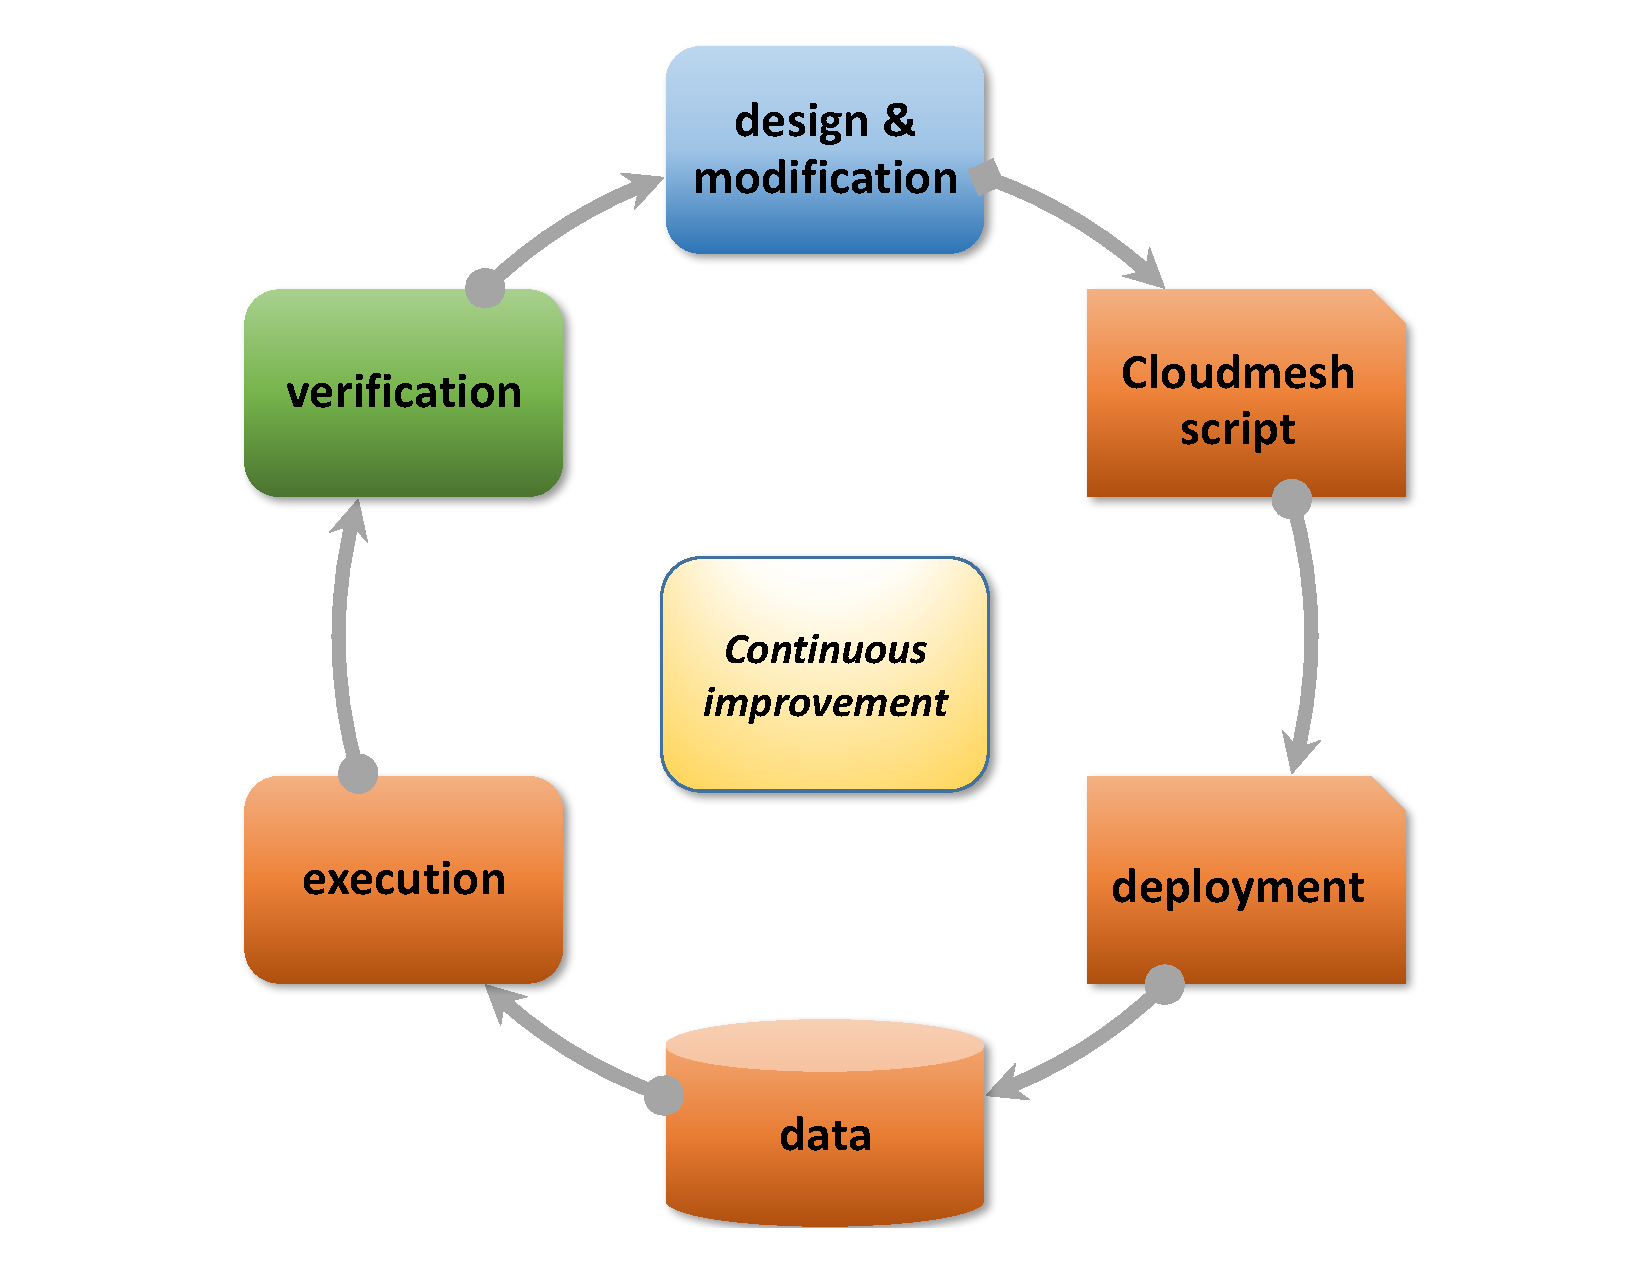
\includegraphics[width=1.0\columnwidth]{images/nist-devops-1.pdf}
  \caption{Continuous improvement while using cloudmesh interactively.}
  \label{F:NIST-devops-1}
\end{figure}


Figure \ref{F:NIST-devops-1} depicts a high level overview of the cyclic workflow
associated with a single application for a specific dataset. Starting
with a Cloudmesh Script that allocates resources and then deploys the
necessary software and desired dataset. The analytics component
executed is then executed. Upon verification of the results and
modification of compnenets as needed the process repeats. This
continues iteratively until the desired results are achieved. Tests at
the end that verify certain results will be used to verify if the
resulting run was successful. If not they are flagged and a
notification is send to the maintaining team. New big data tests can
be integrated into the set of benchmarks tested and the they can be
evaluated based continuously or upon change.


This behaviour is augmented in Figure~\ref{F:NIST-devops-2} with the integration of the
data repositories that are used to manage and maintain the scripts,
the playbooks and the data. While the scripts are simple cloudmesh
scripts to drive a particular application, we envision that most roles
are published as ansible roles to be integrated in application
specific playbooks. Playbooks exists for the phases of the execution

\begin{description}
\item[Phase 0:] start of the integrated application verification
\item[Phase 1:] setup of the infrastructure 
\item[Phase 2:] deployment of the platform and application
\item[Phase 3:] running a test on a specific data set.
\item[Phase 4:] verification of the result
\end{description}


\begin{figure}
  \centering
      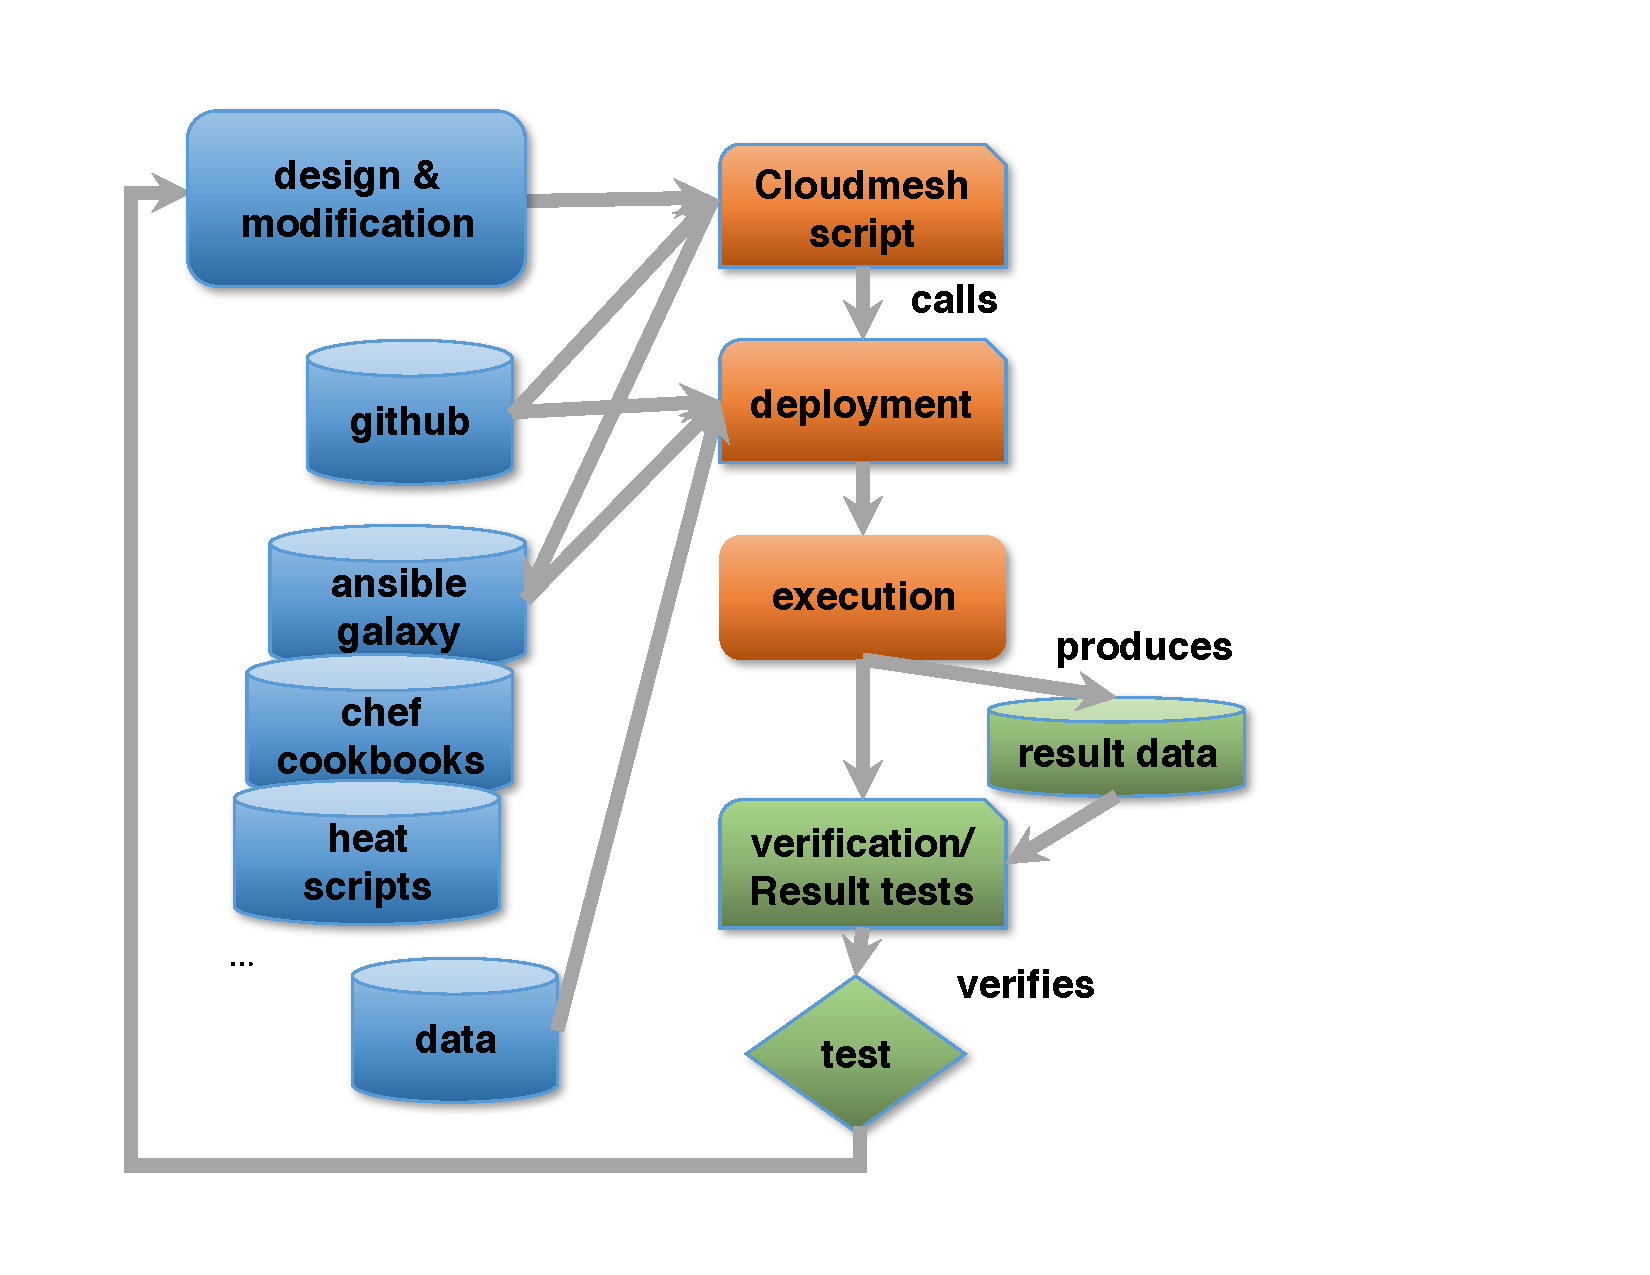
\includegraphics[width=0.8\columnwidth]{images/nist-devops-2.pdf}
  \caption{Interaction of the continuous improvement steps with
    various databases while using ansible deployment scripts.}
  \label{F:NIST-devops-2}
\end{figure}




\section{Provisioning Machines}



The first step in a data processing pipelines is the
provisioning/allocation of compute resources. These can be physical
machines or, increasingly common and accessible, virtual
machines. There are several major technologies that support this
infrustructure as a service paradigm. Some notable ones include Amazon
EC2, Microsoft Azure, Google Compute Engine, and Chameleon Cloud.


Part of our work has been in developing the cloudmesh client, which is
a lightweight client interface of accessing heterogeneous clouds,
clusters, and work- stations right from the users computer. The user
can man- age her own set of resources she would like to utilize. Thus
the user has the freedom to customize their cyber infras- tructure
they use. Cloudmesh client includes an API, a command-line client, and
a command-line shell. It strives to abstract backends to databases
that are used to manage the workflow utilizing the different
infrastructure and also the services. Switching for example to stage
virtual machines from OpenStack clouds to amazon is as simple as
specify- ing the name of the cloud. Moreover, cloudmesh client can be
installed on Linux, MacOSX, and in future Windows.  Currently
cloudmesh supports backends to SLURM, SSH, OpenStack, AWS, and
Azure. Using cloudmesh, users can migrate accross infrustructure
service providers relatively seemlessly.


\begin{figure}[htb]
  \centering
     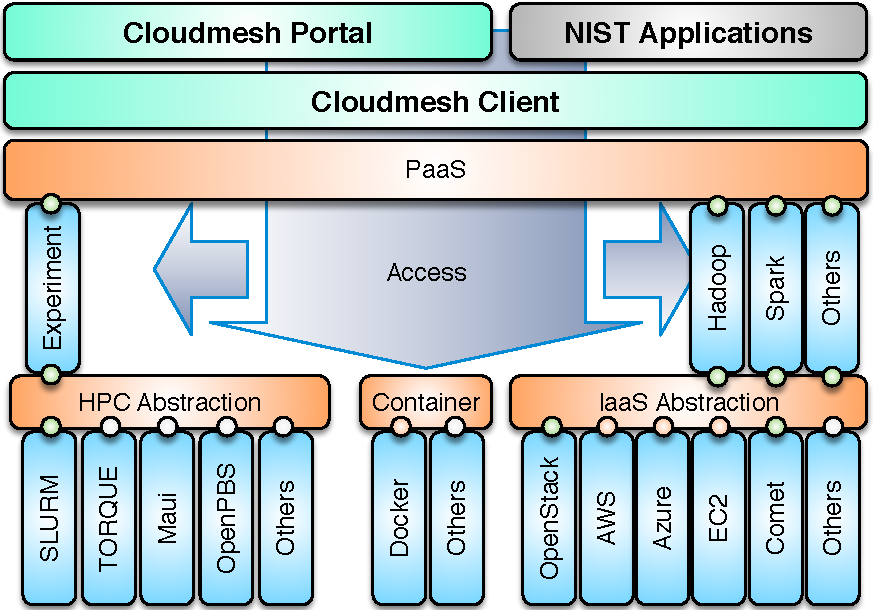
\includegraphics[width=1.0\columnwidth]{images/cloudmesh-arch-1.pdf}
  \caption{Cloudmesh layered architecture.} 
  \label{F:cloudmesh-arch}
\end{figure}


Figure~\ref{F:cloudmesh-arch} describes the architecture of Cloudmesh Client.

%\section{Deployment and Configuration of Software}
\section{Deployment and Configuration}

The second step of the pipelines consists of deploying the desired
software onto newly allocated resources. At this point, nodes may be
available, but are in their initial state, which needs to be updated
by installing and configuring software.


DevOps tools aim to support this component. One significant benefit is
the conceptualization of {/em code-as-infrastructure}, that is the
definitions of the desired state of the clusters are defined in text
files that can be checked into a version control system and tested.

\subsection{DevOps Tools}

The following table provides a short overview of several notable
DevOps tools. These tools allows the state of a cluster to be defined
at various levels. Some (such as Ansible, SaltStack) primarily operate
at the level of software deployment and configuration of a preexisting
cluster, while others (i.e. Juju, NixOps) additionally provide support
for allocating the compute resources. Another factor is the
interaction with the cluster via pushing the desired state to the
nodes, or having the nodes run an agent that pulls the state
definition and then evaluates it locally. Finally, the desired state
is either declaratively defined, where the tools determines the steps
required to achieve the state, or imperatively, where the
user/developer is responsible.


\begin{table*}[htb]
  \label{T:devops-tools}
  \caption{List of notable DevOps tools.}
  \begin{center}
    \begin{small}
      \begin{tabular}{|l|l|l|l|l|}
        \hline
        \blue \textbf{Tool} & \blue \textbf{Developer} & \blue \textbf{License} & \blue \textbf{Method} & \blue \textbf{Approach}
                                                                                                          \tabularnewline \hline

% https://www.ansible.com/
% https://www.chef.io/chef/
% https://puppet.com/
% https://cfengine.com/
% https://saltstack.com/
% https://pressly.github.io/sup/
% http://www.fabfile.org/
% http://inedo.com/otter
% https://jujucharms.com/
% https://nixos.org/nixops/

Ansible   & Ansible Inc.    & GPLv3            & Push      & Declarative            \tabularnewline \hline
Chef      & Chef            & Apache v2        & Pull      & Imperative             \tabularnewline \hline
Puppet    & Puppet          & GPL, Apache      & Pull      & Declarative            \tabularnewline \hline
CFEngine  & CFEngine AS     & GPLv3            & Pull      & Declarative            \tabularnewline \hline
SaltStack & Thomas Hatch    & Apache v2        & Push+Pull & Declarative+Imperative \tabularnewline \hline
Sup       & Pressly, Inc    & MIT              & Push      & Imperative             \tabularnewline \hline
Fabric    & Jeffrey Forcier & Open Source      & Push      & Imperative             \tabularnewline \hline
Otter     & Inedo           & Proprietary      & Push      & Declarative+Imperative \tabularnewline \hline
Juju      & Canonical       & Affero GPL, LGPL & Push      & Declarative            \tabularnewline \hline
NixOps    & NixOS Community & GPLv3            & Push      & Declarative            \tabularnewline \hline

      \end{tabular}
    \end{small}
  \end{center}
\end{table*}


Several of these tools may be used to showcase different capabilities:


\begin{description}

\item[Ansible] YAML-based declarative descriptions of the desired
  state of the system. The description is used to generate a Python
  program that is pushed over SSH to each node, where it is then run
  to modify the system.

\item[Chef] A Ruby Domain Specific Language for defining sets of
  actions (or {/em recipes}). These recipes are pulled onto the
  managed nodes from a configuration server.

\item[Juju] Focuses on connecting services together, using arbitrary
  tools to bring a system to the desired state.

\item[NixOps+NixOS] Resource allocator (EC2, GCE, Azure) for NixOS
  nodes. Once started, the nodes are brought to the desired state by
  interpreting a configuration file which declaratively defines the
  desired state of the node.

\end{description}


\subsection{Concepts}

One of our design principles is to allow the user to use whichever
technologies they are most familiar with. Therefore we do not wish to
constrain them into using a specific DevOps technology such as Ansible
or Chef. Additionally, there are many deployment definitions for
various technologies publically available for these deployment
software, as well as private definitions housed by whichever company
developed them.


\begin{description}

\item[Cluster] A cluster is a collection of virtual machines that can
  be references as a group. Methods acting on the virtual cluster are
  restricted to adding and removing instances. This layer is
  responsible for allocating and deallocating resources (i.e. starting
  and stopping the instances).


\item[Stack] A stack defines how a particular technology is to be
  deployed. This uses deployer plugins to support using Ansible Roles,
  Chef Recipes, NixOS configurations, etc. The core concept is that a
  Stack represents a single technology, such as Hadoop, or Spark, or
  HBase. One of the desired properties of Stack evaluation is
  idempotence. Evaluating a given Stack on a node multiple times
  should have the exact same effect on the state of the system as
  evaluating it once.


\item[Composition] A Composition is a group of Stacks that as a whole
  represent the deployment of a group of technologies. For instance
  Figure FIXME shows that in order to provide Fingerprint Matching as
  a service, one would need a Web stack, a Fingerprint stack, and the
  Hadoop stack.

  \begin{figure}
    \centering
    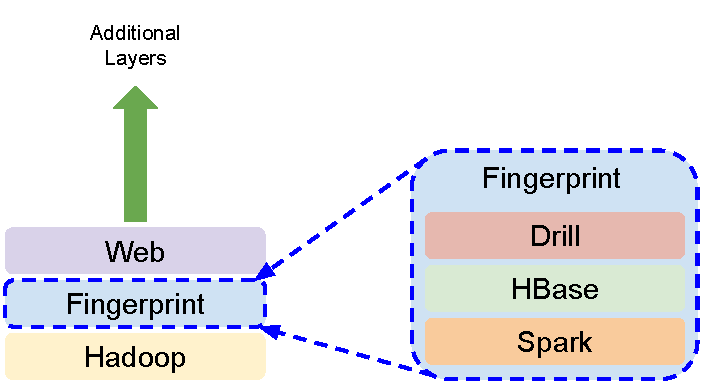
\includegraphics[width=1\columnwidth]{images/cloudmesh-stack-composition.pdf}
    \caption{Multiple stacks may be composed. Here, the
      {\it Fingerprint} stack is a composition of the Apache
      {\it Drill}, {\it HBase}, and {\it Spark}
      stacks. The {\it Fingerprint} stack is then included as a layer withing
      another composition built upon {\it Hadoop} and extended with the
      {\it Web} layers. The {\it Web} layer itself may be composed
      of other layers.
      \label{F:stack-composition}}
  \end{figure}

  Figure~\ref{F:stack-composition}. Fingprint Stack composed with Hadoop and Web stacks to
  provide Fingerprinting-as-a-Service. Note that Stacks can also be
  Compositions


  One crucial concept is that Stacks and Compositions are mutually
  recursive: a Composition is composed of at least one Stack, and each
  stack itself be a composition.


\item[Link] A Link allowes services to introspect properties of the
  virtual cluster and other Stacks at the time of deployment. For
  example, during the deployment of Apache Hadoop, the Hadoop Stack
  needs to determine the address of the nodes running the Zookeeper
  service, as well as the port on which Zookeeper is
  exposed. Currently this information is maintained by hand, which
  causes deployments to be very sensistive to how dependent
  compositions are configured. The goal for Linking is to propagate
  this information throughout the Stack Composition dependency graph
  as needed.


\item[Deployment/Evaluation] A Deployment defines DevOps
  application-specific interface to evaluate Compositions.  Figure
  FIXME shows how the sample Fingerprint service stack shown in Figure
  FIXME may be evaluated. First the Daemon Watcher stack is deployed,
  as it is required by Hadoop. Although Java Stack is required for
  Hadoop, Spark, HBase, and Drill, it should only be evaluated once
  per node. The Fingerpring and Web stack may potentially be evaluated
  in parallel. The semantics of the parallel evaluation is not well
  understood at the moment though.


  
  \begin{figure}
    \centering
    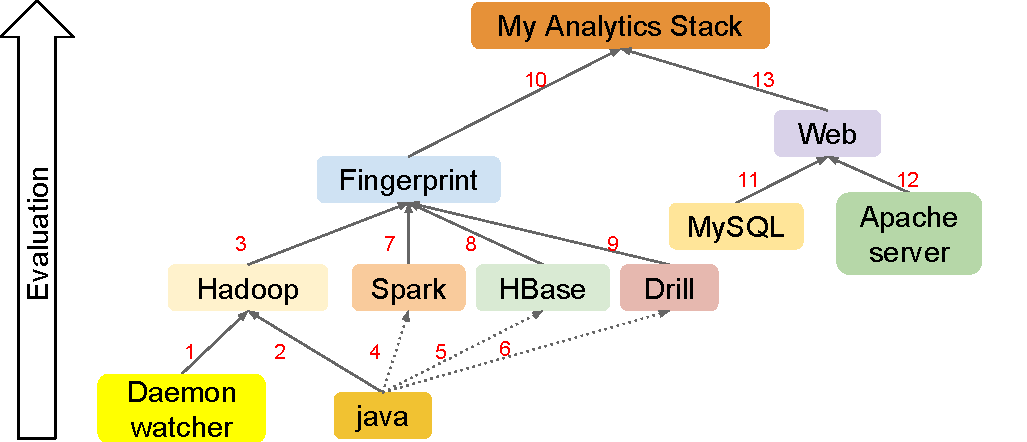
\includegraphics[width=1\columnwidth]{images/cloudmesh-stack-graph.pdf}
    \caption{Evaluation of a stack.
      The {\it My Analytics Stack} is composed of the {\it Fingerprint} and {\it Web} layers.
      These in turn are themselves compositions.
      Numbers indicate order of evaluation.
      While {\it spark}, {\it hbase}, and {\it drill} depend on {\it java}, 
      re-evaluation (\textit{4} - \textit{6}) is not problematic due to the idempotency property.
      \label{F:stack-graph}}
  \end{figure}


  Figure~\ref{F:stack-graph}. Evaluation of a Stack shown as a dependency graph.


\end{description}


\subsection{Design Principles}

\begin{description}

\item[Client based.] As a client, the cloudmesh program requires no
  special privileges to run. This adheres to the principle of least
  priviledge in an attempt to minimize security issues. The program
  runs locally end exits completely once the user terminates it.


\item[Command Shell and Command Line Interface.] The enables scripting
  with cloudmesh as a way of automating virtual cluster deployment and
  tear down.


\item[Plugin Architecture.] The purpose of the plugins is to allow
  users to use the deployment tools they are most familiar with,
  without constraining them to a specific technology. Additionally, a
  desired outcome of this design is increased code sharing and reuse.


\item[REST API.] The goal here is that the client may be used to
  support service-based deployments, in scenarios that warrent it.


\item[Layered Architecture.] The layered architecture, as shown in
  Figure~\ref{F:cloudmesh-arch}, is intended to facilitate development
  and integration of different components that are not currently
  supported. For example, adding Docker support exposes a Docker layer
  that may be used to launch containers in a similar fashion to
  OpenStack virtual machines.


\item[Management Framework.] The supports management of allocated
  resources, allowing starting, stopping, restarting, reinitializing,
  etc.


\item[Database Agnostic.] The state of various components is stored in
  a database. Currently this is an SQLite database, but access to the
  database all passes through a dedicated module. The hope is that, if
  needed, the database backend may be parameterized to support others
  such as MariaDB, PostgreSQL, MongoDB, etc.

\end{description}


\subsection{REST API Development}

As described elsewhere, one of our goals is to provide a
Representational State Transfer (REST) API for cloudmesh. This would
enable web services to more easily use Cloudmesh to provide users with
the ability to use and manage virtual clusters.  REST is a well
understood and widely used approach for designing and developing
service-based APIs. Additionally the semantics of HTTP methods in a
REST context are defined.


Table~\ref{T:rest} shows an initial draft of the Cloudmesh REST
API. These show resources and how the HTTP methods may be used to
manage virtual clusters, stack compositions and deployments, and HPC
experiments.


\begin{table*}[htb]
  \caption{Selected Service Description. Items prefixed with a colon (:) indicate parameters e.g. :id, :?.}
  \label{T:rest}
  \bigskip
  \begin{center}
    \begin{small}
      \begin{tabular}{|l|l|l|}
        \hline
        \blue \textbf{Resource} & \blue \textbf{REST Method} & \blue \textbf{Description}\tabularnewline

%%%%%%%%%%%%%%%%%%%%%%%%%%%%%%%%%%%%%%%%%%%%%%%%%%%%%%%%%%%%%%%% Virtual cluster
\hline \multicolumn{3}{|l|}{\grey\bf Virtual Cluster: /cluster} \tabularnewline \hline
/                         & GET      & List available clusters \tabularnewline \hline
/                         & POST     & Launch a cluster on the provider \tabularnewline \hline
/                         & DELETE   & Delete all available clusters \tabularnewline \hline
/:id                      & DELETE   & Delete and destroy a cluster \tabularnewline \hline
/:id                      & GET      & View the status of a cluster (nodes, node type, etc) \tabularnewline \hline
/:id/properties/:property & GET, PUT & Get/set a property (provider, name, description) of the cluster \tabularnewline \hline
/:id/inventory/:format    & GET      & Obtain an inventory of the cluster \tabularnewline \hline

%%%%%%%%%%%%%%%%%%%%%%%%%%%%%%%%%%%%%%%%%%%%%%%%%%%%%%%%%%%%%%%% Composition
\hline \multicolumn{3}{|l|}{\grey\bf Stack Composition: /stack} \tabularnewline \hline
/                               & GET      & List available compositions \tabularnewline \hline
/                               & POST     & Create a new composition \tabularnewline \hline
/:id                            & GET      & Show information about the composition \tabularnewline \hline
/:id                            & DELETE   & Delete a composition \tabularnewline \hline
/:id/name                       & GET, PUT & Get/set the name of the composition \tabularnewline \hline
/:id/add?deployer=:?\&source=:? & POST     & Add a layer to the composition \tabularnewline \hline
/:id/layers                     & GET      & List layers of the composition \tabularnewline \hline
/:id/layers/:id                 & DELETE   & Delete the layer of the composition \tabularnewline \hline

%%%%%%%%%%%%%%%%%%%%%%%%%%%%%%%%%%%%%%%%%%%%%%%%%%%%%%%%%%%%%%%% Stack Deployment
\hline \multicolumn{3}{|l|}{\grey\bf Stack Deployment: /stack} \tabularnewline \hline
/                         & GET  & List the available stacks with discription \tabularnewline \hline
/:id/deployments/:cluster & POST & Deploy a stack onto a cluster \tabularnewline \hline
/:id/status               & GET  & Current status \tabularnewline \hline
/:id/deployments/:cluster & GET  & Current status on given cluster \tabularnewline \hline

 %%%%%%%%%%%%%%%%%%%%%%%%%%%%%%%%%%%%%%%%%%%%%%%%%%%%%%%%%%%%%%%% Batch
\hline \multicolumn{3}{|l|}{\grey\bf Batch Experiments: /hpc} \tabularnewline \hline
/                          & GET    & List all jobs started with the run command \tabularnewline \hline
/:id                       & DELETE & Deletes the experiment with the given id \tabularnewline \hline
/run?script=:?\&cluster=:? & POST   & Submits an experiment to the named cluster \tabularnewline \hline
/:id/status                & GET    & Returns the status of the job started with the run command \tabularnewline \hline

      \end{tabular}
    \end{small}
  \end{center}
\end{table*}



\section{Ecosystem Analysis}

We believe that big data ecosystem consists of various software,
applications and datasets on different platforms. To understand
current activities on big data projects and provide recommended
software components (roles) in big data, we conduct analysis on big
data projects 1) from community (i.e. github), 2) and academia
(i.e. indiana university) regarding to the following entities:

\begin{itemize}
\item development language preference
\item library/package/tool dependencies
\item sectors of public dataset source
\end{itemize}

This effort will result in building recommended software components
(roles) which supports most of functionalities in a given big data
applications.

\subsection{Analysis on Big Data Projects from Community}

Github.com has been used to provide version control and manage source
code development along with diverse collaborators across
countries. The popularity of github as a collaboration tool has been
significantly increased and 4,995,050 repositories exist as of
12/27/2016 with 20-30 thousands daily added repositories. To
understand trends on big data software development from community, we
conducted a survey of github repositories regarding to big data
applications and tools. Every github repository has a description of a
project and we searched them using topic keywords. For example, we
collected github repositories for Face Detection with search keywords;
face detection, face recognition, human detection, and person
detection to conduct a survey on a series of questions regarding to 1)
A development language distribution, 2) dependency of libraries and
packages, and 3) sectors of public dataset. Actual source code of
public github repositories are evaluated with the survey query data
available on
\url{https://github.com/lee212/bd_stats_from_github}. There are six
topics of NIST Collection used in this analysis where N1: Fingerprint
Matching, N2: Face Detection, N3: Twitter Analysis, N4: Data
Warehousing, N5: Geographic Information Systems, and N6: Healthcare
Data. In addition, a list of recommended components (roles) is created
based on the survey results.

\subsubsection{Language Preference}

TODO
Topic
	C++
	Python
	Java
	Matlab
	JS
	C\#
	C
	R
	Ruby
	Scala
	Count
	Fingerprint
	15%
	11%
	13%

	20%
	3%

	16%
	8%
	0%
	1%
	5%
	43

	FaceDetection
	26%
	21%
	12%
	9%
	7%
	5%
	2%
	2%
	1%
	.02%
	538

	Twitter
	2%
	35%

	15%
	.6%
	9%
	2%
	1%
	10%
	3%

	1%
	1429
	Warehousing
	3%

	27%
	18%
	2%
	10%
	3%

	1%
	10%
	4%
	1%
	3435

	Geographic
	5%
	15%
	27%
	4%
	15%
	3%

	5%
	7%
	3%

	16%
	6487
	Healthcare
	2%
	13%

	19%
	2%
	14%
	5%
	1%
	10%
	6%
	2%
	132

	Table ?:  Language Distribution of Topics related to those in the NIST collection on Github, Count is an average number of github repositories.


        The repository statistics indicate that C++, Python and Java
        are most common languages among the NIST collection (Table 1),
        although Matlab is dominant in the fingerprint.


\subsubsection{Package/Library/Tool Dependencies}

We also notice that scientific python packages are commonly used to
enable numerical computation, data analysis and visualization for
these big data applications (Figure 1), whereas there are dependent
packages for each project (Table 2). Tweepy, twitter API, is used in
the twitter live analysis projects with NLTK, the natural language
processing toolkit to complete sentiment analysis with streaming data,
tweets. Similarly, GIS projects use particular libraries for spatial
analysis such as geopy and shapely. New trends in software development
packages and libraries are observed, for example, deep learning python
packages e.g. caffe or theano have added recently to github
repositories. Statistics (tables 3) show that popular github
repository examples related to the six nist projects started in
2016. Each github project has different language preferences with
various libraries and packages however similar trends are observed,
for example, deep learning software such as Keras, Theano, mxnet and
Caffe are adopted among multiple projects.



  

Figure FIXME: Python Packages used in NIST Collection on Github

Python Package
	Description
	N1
	N2
	N3

	N4
	N5
	N6
	cv2
	OpenCV
	+
	+
	 
	 
	 
	 
	skimage
	Image Processing
	 
	+
	 
	 
	 
	 
	PIL
	Python Imaging Library
	 
	+
	 
	 
	 
	 
	caffe
	Deep Learning
	 
	+
	 
	 
	 
	 
	nltk
	Natural Language Toolkit
	 
	 
	+
	 
	 
	 
	tweepy
	Twitter for Python
	 
	 
	+
	 
	 
	 
	BeautifulSoup
	Screen-scraping library
	 
	 
	+
	+
	 
	 
	gensim
	Topic Modelling
	 
	 
	+
	+
	 
	 
	geopy
	Geocoding library
	 
	 
	 
	 
	+
	 
	shapely
	Geometric Analysis
	 
	 
	 
	 
	+
	 
	django
	Web framework
	 
	 
	 
	+
	 
	+
	Table FIXME: Additional Python Packages found in NIST
        Collection where N1: Fingerprint Matching, N2: Face Detection,
        N3: Twitter Analysis, N4: Data Warehousing, N5: Geographic
        Information Systems, and N6: Healthcare Data



Additional packages or libraries (table FIXME) are not mandatory to provide in a default set of big data suite but it is necessary to see the dependency with a particular application. The choice of applications affects the dependency tools.


Title
	Description
	Language
	Start Date
	Popularity
	Dependency
	OpenFace
	an  open  source  facial   behavior analysis toolkit
	c++
	March, 2016
	725 (305)

	OpenCV,                dlib,
boost, TBB
	Picasso  face
detection transformation
	An  Android  image   transformation library providing cropping above Face Detection (Face Cen tering) for Picasso
	Java
	July, 2016
	528 (56)
	Square Picasso
	MTCNN
face               detection alignment
	Joint Face Detection and Alignment using Multi-task Cascaded Convolutional Neural Networks
	Matlab
	September, 2016
	226 (162)
	Caffe,  Pdollar toolbox
	facematch
	Facebook Face           Recognition
wrapper
	JavaScript
	January, 2016
	132 (41)

	fbgraph,           request,
body-parser,             express
	mxnet mtcnn face detection
	MTCNN face detection
	Python
	October, 2016
	99 (47)
	OpenCV, mxnet
	Table FIXME: Example Projects Recently Created Regarding to Face Detection


\subsubsection{Datasets }

Finding relevant datasets for particular applications is another
challenge for the big data ecosystem because of its difficulty of
collecting data from multiple sources (Kim, Trimi, and Chung, 2014),
complexity and diversity (Hashem et al., 2015). Community contributed
lists of public datasets (Cohen and Lo,2014) provide structured
information with a specific location to access data and a category to
describe itself. We intend to generate linked json data for datasets
and applications in big data ecosystem based on these lists because it
connects scattered data and software in an organized way. Table FIXME
shows the data source from different sectors, academia(.edu or .ac),
government(.gov), organization(.org), industry(.com or .net), and
international(country code in suffix), among the seven topics of the
lists. Entire topics are available online:
\url{https://github.com/lee212/bd_datasets}.


Topic
	Academia
	Government
	Organization
	Industry
	International
	Total
	GIS
	1
	3

	5
	9
	5
	23

	Healthcare
	0
	6
	3

	1
	1
	11
	Image Processing
	11
	0
	4
	2
	5
	18
	Natural Language
	7
	0
	8
	7
	6
	26
	Social Networks
	8
	0
	7
	5
	5
	24
	Climate/Weather
	2
	6
	3

	2
	4
	16
	Energy
	2
	2
	5
	1
	5
	15
	Table FIXME:  Public Dataset of acamedia, government, organization, industry and international from the community list

\subsection{Analysis on Big Data Projects from Academia}

At Indiana University, Big Data Analytics and Applications (BDAA) and
Big Data Open Source Software Projects (BDOSSP) have been offered in
2015 and 2016 according. During these semesters, students have asked
to complete a course project with big data software, tools and
datasets. The statistics for languages, software, and dataset are
provided in this section.


\subsubsection{Language Preference}

Class
	Java
	Python
	R
	C\#
	Projects Count
	Fall ’15
	6
	29
	10
	1
	49
	Spring ’16
	11
	16
	1
	0
	37

	Fall ’16*
	2
	146
	7
	0
	190
	Table  FIXME:  Language Distribution for Big Data Classes from Indiana University
(* Numbers in Table don’t sum up to total count - need to confirm)


\subsubsection{Package/Library/Tool Dependencies}

We had 37 final projects from Big Data Open Source Project Spring 2016
and Table FIXME shows that packages/tools/libraries used in the class
projects. Apache Hadoop is mostly used in conducting data analysis
with a database support from HBase, Hive and HDFS. Python was the most
preferred language in the course projects which resulted in high use
of Spark in data processing with the python library, pyspark. One
another observation is that Ansible, software deployment tool, had
offered as a method of project deployment to ensure reproducibility.





Package
	Type
	Use
	Language
	Count
	Numpy
	library
	data management
	Python
	13

	Pandas
	library
	data management
	Python
	10
	Mongodb
	database
	NoSQL
	C++
	10
	Matplotlib
	library
	visualization
	Python
	8
	scikit-learn
	library
	machine learning
	Python
	7
	Scipy
	library
	data management
	Python
	6
	Hadoop
	framework
	framework
	Java
	6
	Nltk
	library
	NLP
	Python
	5
	ggplot1
	library
	visualization
	R
	4
	IPython Notebook
	tool
	web interface
	Python
	4
	Tableau
	tool
	visualization
	C++
	4
	seaborn
	library
	visualization
	Python
	3

	rstudio
	tool
	development IDE
	R
	3

	Spark
	framework
	in-memory processing
	Scala
	3

	MPI
	framework
	parallel processing
	C, C++, Fortran
	2
	Table FIXME: List of Top 15 Tools/Libraries/Packages used in Big Data Class Fall 2015, count indicates a number of class projects that use a particular tool/library/package


Package
	Type
	Use
	Language
	Count
	Hadoop
	framework
	parallel processing
	Java
	31

	Ansible
	tool
	deployment
	Python
	26
	Spark
	framework
	in-memory processing
	Scala
	14
	HBase
	database
	NoSQL
	Java
	12
v	Pig
	language
	data abstraction
	Java
	11
	Hive
	database
	SQL
	Java
	7
	MongoDB
	database
	NoSQL
	C++
	7
	Mahout
	library
	machine learning, data minig
	Java
	4
	MLLib
	library
	machine learning
	Java
	4
	OpenCV
	library
	computer vision
	C++
	3

	Zookeeper
	framework
	directory service
	Java
	3

	Tableau
	tool
	visualization
	C++
	3

	D3.js

	tool
	visualization
	Javascript
	2
	MySQL
	database
	SQL
	C++
	2
	HDFS
	database
	distributed filesystem
	Java
	2
	Table FIXME: List of Top 15 Tools/Libraries/Packages used in Big Data Class Spring 2016, count indicates a number of class projects that use a particular tool/library/package


Package
	Type
	Use
	Language
	Count
	Matplotlib
	library
	visualization
	python
	88
	Pandas
	library
	data management
	python
	79
	Numpy
	library
	data management
	python
	65
	Scipy
	library
	data management
	python
	24
	Requests
	library
	http tool
	python
	22
	xlrd
	library
	MS Excel
	python
	10
	pillow
	library
	Imaging Library
	python
	9
	scikit-learn
	library
	machine learning
	python
	9
	seaborn
	library
	visualization
	python
	8
	nltk
	library
	language processing
	python
	6
	geopy
	library
	geospatial tool
	python
	5
	pyOpenSSL
	library
	OpenSSL
	python
	5
	patsy
	library
	statistics
	python
	5
	bokeh
	library
	visualization
	python
	4
	ploty
	library
	visualization
	python
	4
	Table FIXME: List of Top 15 Tools/Libraries/Packages used in Big Data Class Fall 2016, count indicates a number of class projects that use a particular tool/library/package


\subsubsection{Datasets}

There were 49 class project in Big Data Analytics and applications Fall 2015, and use of 27 dataset are observed. Public dataset from industry was mainly used (44%) due to the interest on analytics from kaggle and twitter and availability e.g. amazon reviews and yelp reviews.


Class
	Government
	Organization
	Industry
	Academia
	International
	Total
	Fall ‘15
	3

	5
	12
	7
	0
	27
	Spring ‘16
	6
	8
	10
	6
	1
	30

	Fall ‘16
	

	

	

	

	

	

	Table FIXME: Dataset sectors of academia, government, organization and industry from Big Data Classes at Indiana University * Fall ‘16 will be added



\section{Selected Applications}

\subsection{Fingerprint Matching}

Implementation repository (link to GitHub)

\subsubsection{Description}

Fingerprint recognition refers to the automated method for verifying a match between two fingerprints and that is used to identify individuals and verify their identity. Fingerprints (Figure 1) are the most widely used form of biometric used to identify individuals.
 Example fingerprints 

Figure 1 Example fingerprints


The automated fingerprint matching generally required the detection of different fingerprint features (aggregate characteristics of ridges, and minutia points) and then the use of fingerprint matching algorithm, which can do both one-to- one and one-to- many matching operations. Based on the number of matches a proximity score (distance or similarity) can be calculated.


The goal for this project is: given a set of {/em probe} and {/em gallery}
images, compare the probe images to the gallery images, and report the
matching scores.  The dataset used comprises 54,000 images along with
their metadata. Provided tools include MINDTCT and BOZORTH3, which are
part of the NIST Biometric Image Software (NBIS) release. These two
tools form the core of the application: MINDTCT preprocesses the
images to identify minutae which is used by BOZORTH3 to compute a
match.



The implemented solution uses stack of HDFS, YARN, Apache Spark, Apache HBase, and Apache drill. A Hadoop cluster is deployed and YARN used to schedule Spark jobs that load the images into HBase, process the images, and compute the matches. Apache Drill, with the HBase plugin, can then be used to generate reports.

\subsubsection{Software Stack}

Big Data software packages:

\begin{itemize}
\item Apache Hadoop (YARN)
\item Apache Spark
\item Apache HBase
\item Apache Drill
\end{itemize}

Datasets:
\begin{itemize}
\item NIST Special Database 14 - Mated Fingerprint Card Pairs 2.
\end{itemize}

Domain Specific code (NBIS):
\begin{itemize}
\item MINDTCT
\item BOZORTH3
\end{itemize}


Other tools and technologies:
\begin{itemize}
\item Scala
\end{itemize}

\subsubsection{Deployment Approach}

The resource allocation can be done using Cloudmesh Client.
Next, Cloudmesh Big Data Stack is used to deploy the Big Data software packages.
Finally, some Ansible playbooks deploy and compile a scala program that integrates the Big Data infrustructure with running the domain specific code.

\subsubsection{Development Status}

Complete



\subsubsection{Lessons Learned}

\subsection{Face Detection}

Implementation repository:\\
 \url{https://github.com/futuresystems/pedestrian-and-face-detection}

\subsubsection{Description}

Human detection and face detection have been studied during the last
several years and models for them have improved along with Histograms
of Oriented Gradients (HOG) for Human Detection [FIXME]. OpenCV is a
Computer Vision library including the SVM classifier and the HOG
object detector for pedestrian detection and INRIA Person Dataset [FIXME]
is one of popular samples for both training and testing purposes. This
example shows how to deploy the NIST Human and Face Detection with
INRIA Person Dataset to the cluster where we deployed Apache Spark on
Mesos to train and apply detection models from OpenCV using Python
API. OpenCV Python code runs with Spark Map function to perform
distributed job processing on the Mesos scheduler.
  
  

FIXME Figure 1. Human Detection, original image (left), processed image (right)
  
  

FIXME Figure 2. Face and Eye Recognition with Human Detection (face: blue box, eye: red box, human: green box)


When it comes to deploy applications and build clusters for
batch-processing large datasets, Ansible scripts play a big role such
as installation and configuration towards available machines. Ansible
provides abstractions by Playbook Roles and reusability by Include
statements. We define X application in X Ansible Role, for example,
and use include statements to combine with other applications e.g. Y
or Z. Five Ansible roles are used in this use case to build clusters
for Human and Face Detection with INRIA dataset. The main Ansible
playbook runs Ansible roles in order which looks like:


\begin{verbatim}
* include: sched/00-mesos.yml
* include: proc/01-spark.yml
* include: apps/02-opencv.yml
* include: data/03-inria-dataset.yml
* include: anlys/04-human-face-detection.yml
\end{verbatim}
	

Directory names e.g. sched, proc, data, or anlys indicate BDSS layers like:
\begin{itemize}
\item sched: scheduler layer
\item proc: data processing layer
\item apps: application layer
\item data: dataset layer
\item anlys: analytics layer
\end{itemize}

and two digits in the filename indicate an order of roles to be run. 


It is assumed that virtual machines are created by
virtual-cluster-libs, the command line tool to start VM instances. For
example on OpenStack,

\begin{verbatim} 
vcl boot -p openstack -P $USER
\end{verbatim}

command starts a set of virtual machine instances with a cluster
definition file `.cluster.py`. The number of machines and groups for
clusters e.g. namenodes and datanodes are specified in the file and
Ansible inventory file, a list of target machines with groups, is
generated once machines are ready to use. Ansible roles run to install
applications on virtual clusters.


Mesos role is installed first with Ansible inventory groups for
masters and slaves in which mesos-master runs on the masters group and
mesos-slave runs on the slaves group. Apache Zookeeper is included in
the mesos role so that mesos slaves find an elected mesos leader from
the zookeeper. Spark, as a data processing layer, provides two options
for distributed job processing, batch job processing via a cluster
mode and real-time processing via a client mode. The Mesos dispatcher
runs on a masters group to accept a batch job submission and Spark
interactive shell, which is the client mode, provides real-time
processing on any node in the cluster. Either way, Spark is installed
after a scheduler layer i.e. mesos to identify a master host for a job
submission. Installation of OpenCV, INRIA Person Dataset and Human and
Face Detection Python applications are followed.


\subsubsection{Software Stack}

Big Data software packages

\begin{itemize}
\item Apache Spark
\item Apache Mesos
\item Apache Zookeeper
\item OpenCV (with Python)
\end{itemize}

Datasets:

\begin{itemize}
\item INRIA Person Dataset
\end{itemize}

\subsubsection{Deployment Approach}

Mesos role is installed with two Ansible inventory groups; masters and
slaves where mesos-master runs on the masters group and mesos-slave
runs on the slaves group. Apache Zookeeper is included in the mesos
role and mesos slaves find an elected mesos leader from the
zookeeper. Spark, as a data processing layer, provides two options for
distributed job processing, batch job processing via a cluster mode
and real-time processing via a client mode. The Mesos dispatcher runs
on a masters group to accept a batch job submission and Spark
interactive shell, which is the client mode, provides real-time
processing on any node in the cluster. Either way, Spark is installed
after a scheduler layer i.e. mesos to identify a master host for a job
submission. Installation of OpenCV, INRIA Person Dataset and Human and
Face Detection Python applications are followed.

\subsubsection{Development Status}

Complete

\subsubsection{Lessons Learned}


\subsection{Twitter Analysis}


\subsection{Analytics for Healthcare Data and Informatics}

\section{Spatial Big Data/Statistics/Geographic Information Systems}

\section{Data Warehousing and Mining}

Components (Roles)
Based on the analysis from community and academia, we observed that there are crucial software, dataset and analytics in big data ecosystem. We, therefore, offer deployable first-class roles which enable major functionalities on big data processing and analysis. The software deployment is accommodated with Cloudmesh, Ansible, Chef, Puppet, Salt, OpenStack Heat, Microsoft Azure Template, and Amazon Cloudformation.

\begin{verbatim}
* Framework
   * Hadoop
   * Mesos
* Processing
   * Spark
   * Storm
* Language
   * Pig
   * R
* Database
   * HBase
   * Hive
   * MongoDB
   * MySQL
* Library
   * Mahout
   * nltk
   * MLlib
   * Lucene/Solr
   * OpenCV
* Tools
   * Ganglia
   * Nagios
   * Zookeeper
\end{verbatim}

In detail, table is provided:

\begin{verbatim}
Role Name
	Description
	Type
	Requirement (installation)
	Dependencies
	Distributed
	Example
	Spark
	In-memory data processing application
	processing
	JDK 7+
\end{verbatim}

Maven 3.3.9

	Hadoop (optional)
	Cluster Manager/Executor (Worker node)
	

	hadoop
	Map/Reduce distributed processing framework
	framework
	JDK
SSH
	

	Resource Manager/Node Manager
	WordCount
	Storm
	a real time fault-tolerant and distributed stream data processing system [1]
	processing
	OpenJDK


	ZooKeeper
	Master/Worker
	

	Zookeeper
	Synchronization service for distributed processes
	tool
	JDK 6+
	

	Ensemble (3 servers minimum)

	

	hbase
	NoSQL database for real-time processing
	database
	JDK
	ZooKeeper
	Master/RegionServer
	

	Twitter REST APIs
	Reading Twitter data
	library
	

	OAuth
	

	

	D3, tableau

	Javascript visualization library
	visualization
	

	

	

	

	Nltk
	Natural Language Toolkit
	library
	Python2.7 or 3.2+

	Numpy (optional)
	

	

	AlchemyAPI
	Collecting Tweets
	library
	Mongodb, R (ggplot2)
	

	

	

	OpenCV
	Computer Vision Libraries
	library
	

	

	

	

	Mahout
	Machine learning applications
	library
	JDK
Maven
	hadoop-client
	Via Hadoop, Spark, H20 or Flink
	Naive Bayes (Classification)
K-Means (Clustering)
Recommender
	Lucene/Solr
	Search engine framework
	library
	JRE 1.8+
	

	SolrCloud
	

	MLlib
	Machine Learning Library from Spark
	library
	

	Spark
	

	Logistic regression (Classification)
K-means (Clustering)
	

	

	

	

	

	

	

	





Software Stacks
Cloudmesh is primary, uses BDS under hood.
https://github.com/futuresystems/big-data-stack


Conclusions
Goals
Design principles
Lessons learned




\section*{Acknowledgements}

This work was in part supported by FIXME


% Bibliography

\bibliography{references}
 



\end{document}
